\documentclass[12pt]{article}

% The preceding line is only needed to identify funding in the first footnote. If that is unneeded, please comment it out.
\usepackage{cite}
\usepackage{amsmath,amssymb,amsfonts}
\usepackage{algorithm}
\usepackage{algorithmic}
\usepackage{graphicx}
\usepackage{textcomp}
\usepackage{xcolor}
\usepackage{colortbl}
\usepackage{float}
\usepackage{subcaption}
\usepackage{multirow}

\graphicspath{{../result/}}

\def\BibTeX{{\rm B\kern-.05em{\sc i\kern-.025em b}\kern-.08em
    T\kern-.1667em\lower.7ex\hbox{E}\kern-.125emX}}
\begin{document}

\title{Coursework of Machine learning cousework 2}



\author{Chen Ting Hung} {}
	
\maketitle

\begin{abstract}
This is the report of out machine learning cousework
\end{abstract}

\section{Subtask 1}
Implement ICM for a binary image that you have corrupted with noise, show the result for a set of images with different noise levels. How many passes through the nodes do you need until you are starting to get descent results?\\

a) a set of images\\
\begin{figure}[htb]
\centering
\begin{subfigure}[b]{.48\linewidth}
  \centering
  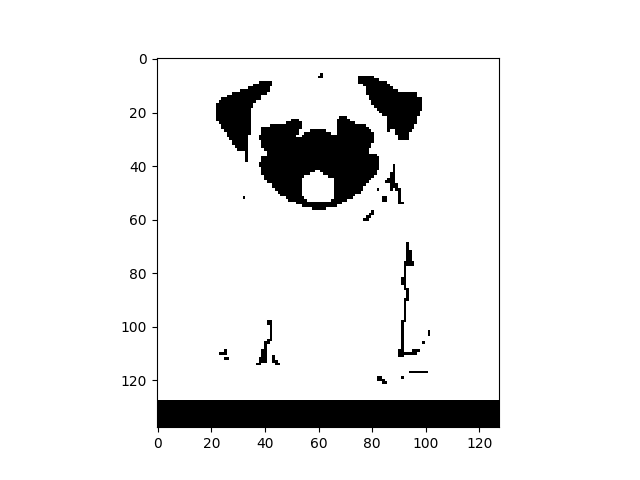
\includegraphics[width=\linewidth]{../result/restore0-1.png}
  \caption{\textbf{\texttt{restore0-1.jpg}}}
\end{subfigure}
\label{fig:1}
\end{figure}

b) How many passes through the nodes\\
we do the three different level of gaussian noises all of propotion are setted as 0.7.\\ 
First time is use 0.1 as varSigma, second time is 0.3 and third time is 0.5.\\
We notice that with the noise larger it might increase the amount of nodes.\\
Finally, we notice that most of the progress will end around passed through 10 nodes.\\

\section{Subtask 4}
What effect does the number of iterations we run the sampler have on the results? Try to run it for different times, does the result always get better?\\

Gibbs sampling is a MCMC algorithm for obtaining a sequence of observations which are approximated from a specified multivariate probability distribution, when direct sampling is difficult. When Gibbs sampling algorithm is executed multiple times, the resulting distribution would converge to the distribution of real samples, which is the reason that why Gibbs sampling is reliable.\\
According to this, before the distribution converging to the real one, the number of iterations would have effect on our results; however, after the convergence, the effect would be much smaller than expected.

\section{Subtask 5}
In machine learning, KL-divergence is used to measure the difference between two probability distributions in the same event space.We assume q(x) as the original distribution, p(x) is the assuming distribution that we used to match q(x).  When the two distribution get much closer, $log{\frac{q(x)}{p(x)}}$will be more equal to 1 and $KL(q(x)||p(x))$
and $KL(p(x)||q(x))$ would get the same answer. However, when it comes to the scenario that $p(x=x_i)=0$ but $q(x=x_i)\neq0$, then $KL(q(x)||p(x))$ would goes infinite while $KL(p(x)||q(x))$ is 0, and in this case KL-divergence is asymmetrical.

\section{Subtask 9}

\end{document}
